\section{Android App}
\label{sec:android_app}

The BiteBound Android application acts as a remote controller and telemetry dashboard, facilitating secure, real-time bidirectional communication with the ESP32-S3 over MQTT. Developed in Kotlin~\cite{kotlin2026} using the Model-View-ViewModel (MVVM) architecture~\cite{maui2026mvvm}, the system separates data and transmission processes from user interface rendering across four architectural layers:

\begin{itemize}
    \item \textbf{Data Layer}: Manages profile persistence via Android SharedPreferences~\cite{android2026sharedpreferences}, telemetry deserialization, command serialization, and local data structures. This layer matches configuration constants, boundaries, and different ball presets to the ESP32 firmware specifications.

    \item \textbf{Network Layer}: Handles connectivity tasks using the HiveMQ client~\cite{hivemq2026mqttclient}. It coordinates SSL/TLS handshakes~\cite{aws2026ssl}, topic subscriptions, automatic reconnection cycles, and message publication.

    \item \textbf{UI State and Logic Layer}: Orchestrated by a central ViewModel that maintains screen states, parses real-time telemetry updates, monitors connection heartbeats, and dispatches command requests.

    \item \textbf{UI Layer (Screens)}: Renders the interface using declarative, stateless composables via Jetpack Compose~\cite{compose2026material3}. It features a configuration screen to initialize parameters (\Cref{fig:android-connection-screen}) and an active gameplay dashboard that displays performance metrics, sensor diagnostics, and a dynamic canvas~\cite{htmlcanvas2026} tracking ball position and velocity (\Cref{fig:android-dashboard-screen}).
\end{itemize}

\begin{figure}[p]
    \centering
    \begin{minipage}[b]{0.48\linewidth}
        \centering
        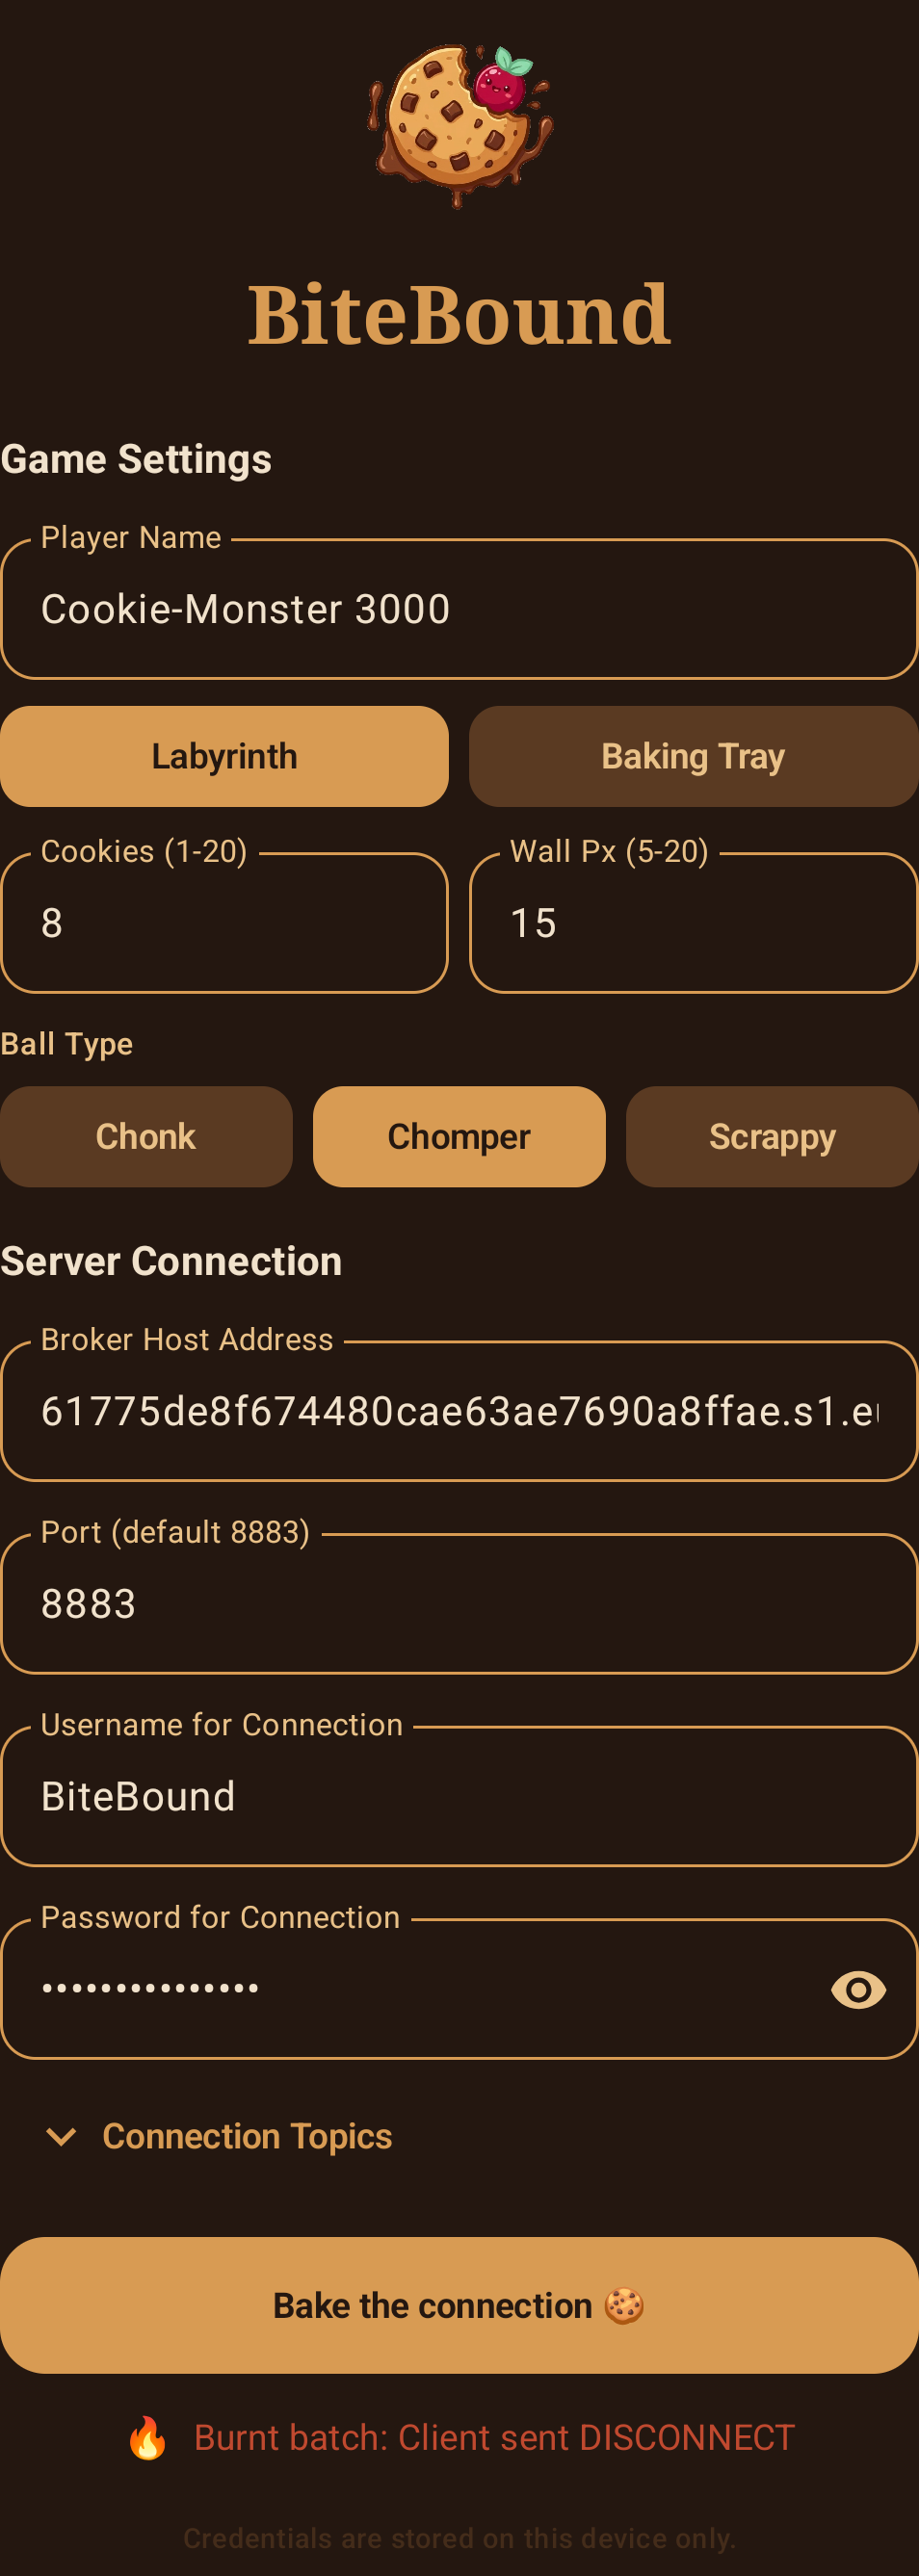
\includegraphics[width=0.8\linewidth]{../assets/android-app-1.png}
        \caption[BiteBound Connection Screen]{Android app connection setup screen for MQTT broker and game configurations.}
        \label{fig:android-connection-screen}
    \end{minipage}
    \hfill
    \begin{minipage}[b]{0.48\linewidth}
        \centering
        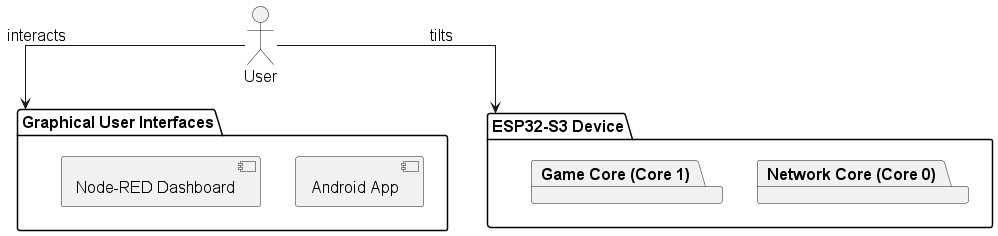
\includegraphics[width=0.65\linewidth]{../assets/android-app-2.png}
        \caption[BiteBound Dashboard Screen]{Android app dashboard displaying real-time telemetry and controller interface.}
        \label{fig:android-dashboard-screen}
    \end{minipage}
\end{figure}